\chapter{Показатели XiYan-SQL в ключевых бенчмарках задачи Text-to-SQL}\label{appendix-A}

\begin{figure}[h]
	\centering
	\begin{subcaptiongroup}
		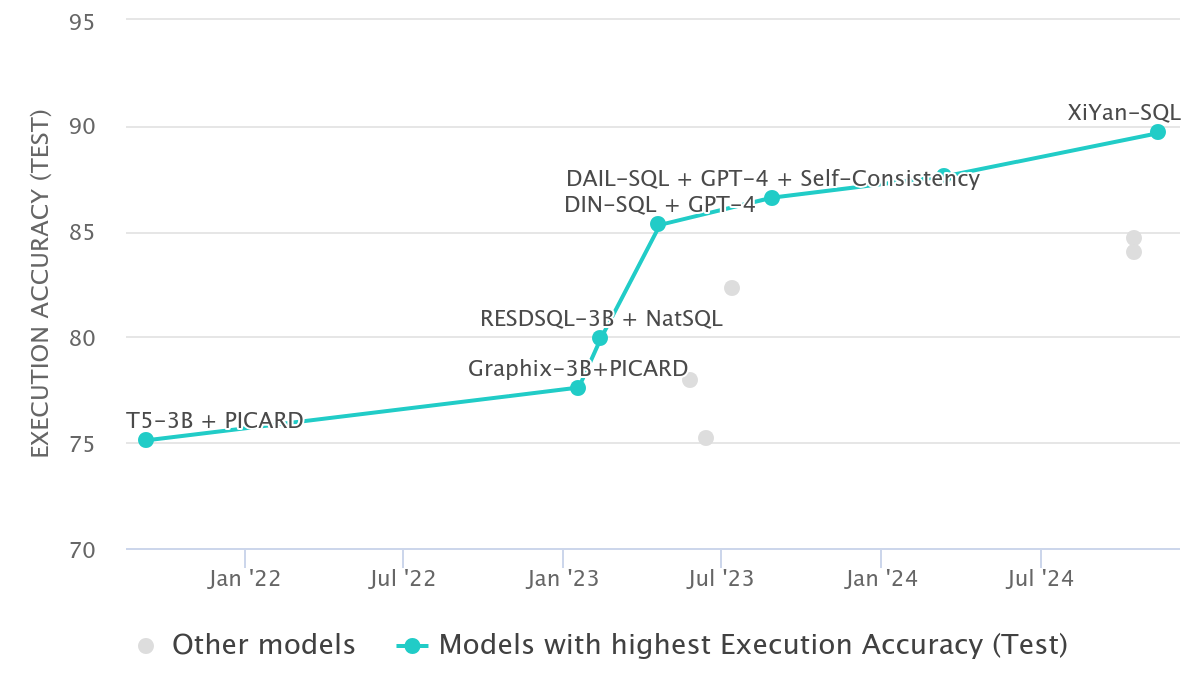
\includegraphics[width=0.85\textwidth]{literature-review/SOTA-Spider.png}
		\caption{Бенчмарк Spider}
		\label{fig:SOTA-Spider}
		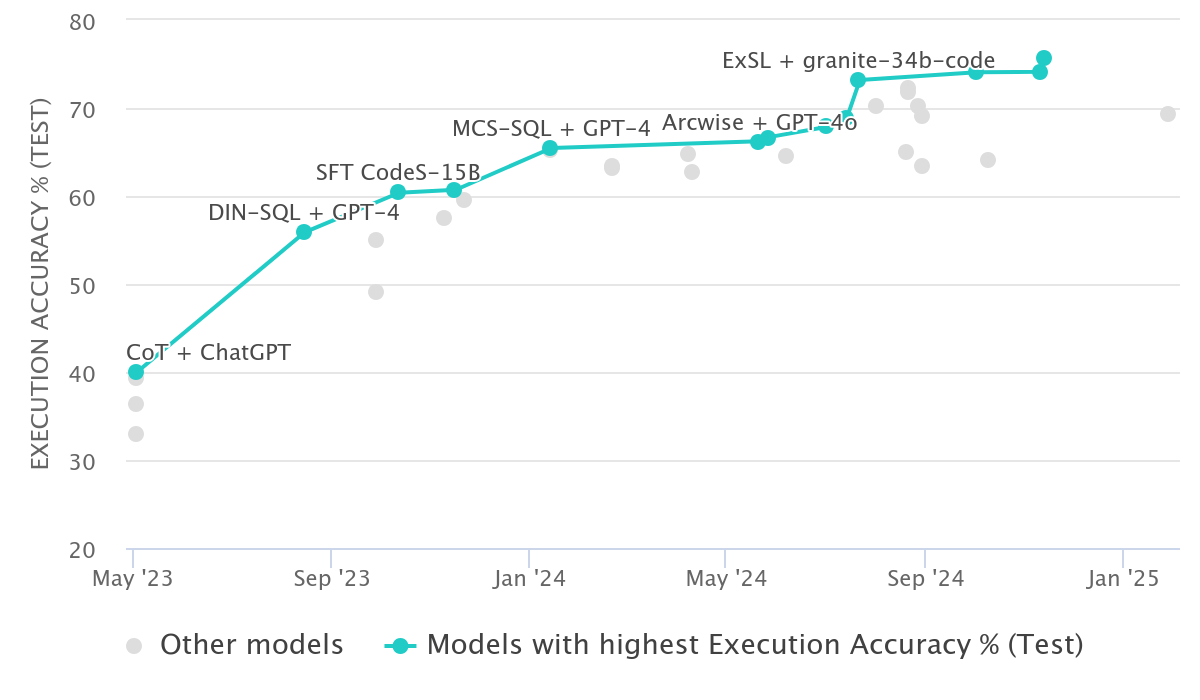
\includegraphics[width=0.85\textwidth]{literature-review/SOTA-BIRD.png}
		\caption{Бенчмарк BIRD}
		\label{fig:SOTA-Bird}
	\end{subcaptiongroup}
	\captionsetup{subrefformat=parens}
	\caption{Графики лидеров на бенчмарках Spider и BIRD}
	\label{fig:SOTA-Spider-Bird}
\end{figure}

%Далее приложения начинаются с новых страниц
\makeatletter
\let\clearpage\oldclearpage
\makeatother

\clearpage

\chapter{Фрагменты программного кода}\label{appendix-B}

\lstinputlisting[
	language=Python,
	label=lst:main_app,
	frame=lines,
	breaklines=true,
	caption={Точка входа в приложение (\texttt{main.py})}
]{4-listings/main.py}

\lstinputlisting[
	language=Python,
	label=lst:user_register,
	float=tb,frame=lines,
	caption=Реализация эндпоинта регистрации пользователя (\texttt{features/users/api.py})
]{4-listings/user_register.py}

\lstinputlisting[
	language=Python,
	label=lst:table_upload,
	float=tb,frame=lines,
	caption=Реализация эндпоинта загрузки таблицы (\texttt{features/tables/api.py})
]{4-listings/table_upload.py}

\lstinputlisting[
	language=Python,
	label=lst:table_preview,
	float=tb,frame=lines,
	caption=Реализация сервисной функции для получения превью таблицы (\texttt{services/table\_service.py})
]{4-listings/table_preview.py}

\lstinputlisting[
	language=Python,
	label=lst:nli-core-mock,
	float=tb,frame=lines,
	caption=Реализация модуля-эмулятора ядра NLIDB (\texttt{services/text\_to\_sql\_service.py})
]{4-listings/nli_core_mock.py}

\clearpage

\chapter{Вывод терминала об отчете тестирования прототипа}\label{appendix-C}

\lstinputlisting[
	language=bash,
	label=lst:test_report,
	frame=lines,
	breaklines=true,
	caption={Вывод терминала при запуске тестирования прототипа (\texttt{test-report.sh})}
]{4-listings/test-report.sh}